\begin{enumerate}[label=\thesubsection.\arabic*,ref=\thesubsection.\theenumi]
%
\item Find the area bounded by the curves $\brak{x-1}^2 + y^2 = 1 \text{ and } x^2+y^2=1$.
\label{chapters/12/8/2/2}
\\
\solution
The conic parameters for the two circles can be expressed as
\begin{align}
\begin{split}
	\vec{V}_1 &= \myvec{1&0\\0&1},\
	\vec{u}_1 = \myvec{-1\\0},\
	f_1 = 0,
	\\
	\vec{V}_2 &= \myvec{1&0\\0&1},\
	\vec{u}_2 = \myvec{0\\0},\
	f_2 = -1.
\end{split}
	\label{eq:12/8/2/2/vuf}
\end{align}
On substituting from
	\eqref{eq:12/8/2/2/vuf}
	in
	  \eqref{eq:pair-mat-sing-conic-det}, we obtain
\begin{align}
	\mydet{1+\mu & 0 & -1 \\ 0 & 1+\mu & 0 \\ -1 & 0 & -\mu} = 0
\end{align}
yileding
\begin{align}
	\mu= -1.
\end{align}
Substituting 
	\eqref{eq:12/8/2/2/vuf}
in 
	  \eqref{eq:pair-mat-sing-conic},
	  we obtain
\begin{align}
	\vec{x}^\top\myvec{0&0\\0&0}\vec{x} + 2\myvec{-1&0}\vec{x} + 1 &= 0\\
\implies	\myvec{-2&0}\vec{x} &= -1 
\label{eq:12/8/2/2/chord}
\end{align}
Therefore the intersection of the two circles is a line with parameters
\begin{align}
	\vec{m} = \myvec{0\\1},  \vec{h} = \myvec{\frac{1}{2}\\0}.
\end{align}
	The intersection parameters of the 
	chord in 
\eqref{eq:12/8/2/2/chord}
with the 
first circle in \eqref{eq:12/8/2/2/vuf} is obtained from 
\eqref{eq:tangent_roots}
	as
\begin{align}
	\mu_i= \pm\frac{\sqrt{3}}{2}
\end{align}
Hence the point of intersection are
obtained from
	\eqref{eq:chord-pts}
	as
\begin{align}
	\vec{a}_0 = \myvec{\frac{1}{2}\\[1ex]\frac{\sqrt{3}}{2}}, \vec{a}_2 = \myvec{\frac{1}{2}\\[1ex]-\frac{\sqrt{3}}{2}}.
\end{align}
The desired area of region is given as
\begin{multline}
	2\brak{\int_{0}^{\frac{1}{2}} \sqrt{1-\brak{x-1}^2}dx + \int_{\frac{1}{2}}^{1} \sqrt{1-x^2}dx}\\
		=2\sbrak{\frac{1}{2}\brak{x-1}\sqrt{1-\brak{x-1}^2}+\frac{1}{2}\sin^{-1}\brak{x-1}}_{0}^{\frac{1}{2}}\\
		 +2\sbrak{\frac{x}{2}\sqrt{1-x^2}+\frac{1}{2}\sin^{-1}x}_{\frac{1}{2}}^{1}
	= \frac{2\pi}{3}-\frac{\sqrt{3}}{2}
\end{multline}
See \figref{fig:chapters/12/8/2/2/Fig1}.
\begin{figure}[H]
	\begin{center} 
	    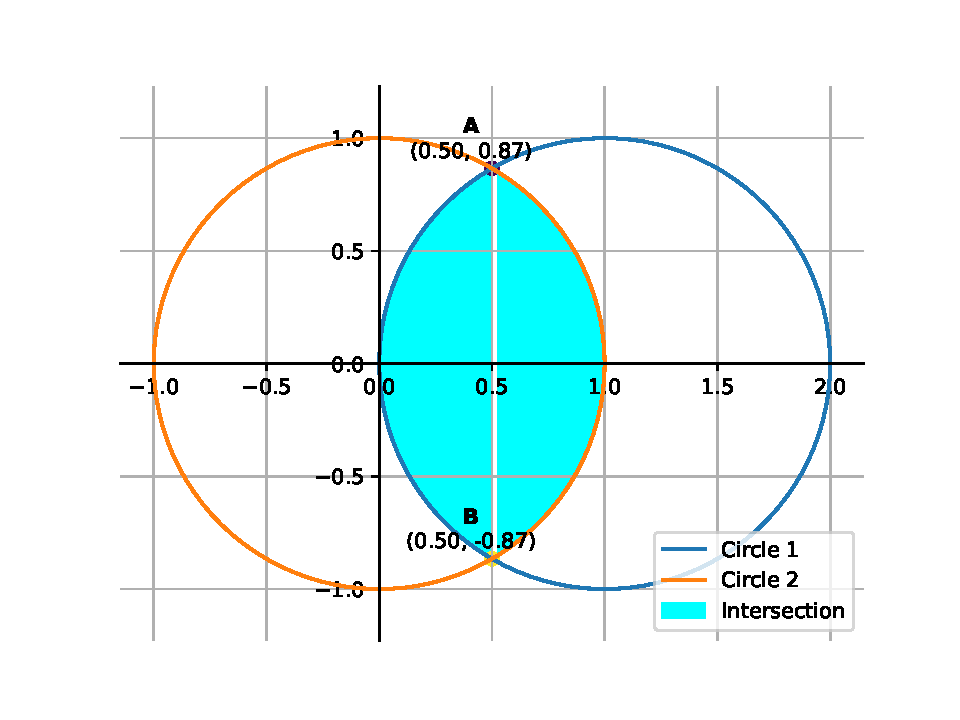
\includegraphics[width=0.75\columnwidth]{chapters/12/8/2/2/figs/fig.pdf}
	\end{center}
\caption{}
\label{fig:chapters/12/8/2/2/Fig1}
\end{figure}



















\item 
	Find the area of the circle $4x^2+4y^2=9$ which is interior to the parabola $x^2=4y$.
\label{chapters/12/8/2/1}
\item 
	Find the area of the circle $x^2 + y^2 = 16$ exterior to the parabola $y^2 = 6x$.
\label{chapters/12/8/3/18}
\item Find the area of the region bounded by the curve $y^2 = 2x\text{ and }x^2 + y^2 = 4x$.
\item
Solve
\begin{align*}
\frac{1}{3x+y}+\frac{1}{3x-y}&=\frac{3}{4}\\ \frac{1}{2(3x+y)}-\frac{1}{2(3x-y)}&=\frac{-1}{8}
\end{align*}
\end{enumerate}
